 % -*- TeX-engine: xetex; eval: (auto-fill-mode 0); eval: (visual-line-mode 1); -*-
% Compile with XeLaTeX

%%%%%%%%%%%%%%%%%%%%%%%
% Option 1: Slides: (comment for handouts)   %
%%%%%%%%%%%%%%%%%%%%%%%

%\documentclass[slidestop,compress,mathserif,12pt,t,professionalfonts,xcolor=table]{beamer}
%
%% solution stuff
%\newcommand{\solnMult}[1]{
%\only<1>{#1}
%\only<2->{\red{\textbf{#1}}}
%}
%\newcommand{\soln}[1]{\textit{#1}}

%%%%%%%%%%%%%%%%%%%%%%%
% Option 2: Slides: (to post)                          %
%%%%%%%%%%%%%%%%%%%%%%%

%\documentclass[slidestop,compress,mathserif,12pt,t,professionalfonts,xcolor=table]{beamer}
%
% % solution stuff
% \newcommand{\solnMult}[1]{#1}
% \newcommand{\soln}[1]{}

%%%%%%%%%%%%%%%%%%%%%%%%%%%%%%%
% Option 3: Handouts, without solutions (post before class)    %
%%%%%%%%%%%%%%%%%%%%%%%%%%%%%%%

 \documentclass[11pt,containsverbatim,handout,xcolor=xelatex,dvipsnames,table]{beamer}

 % handout layout
 \usepackage{pgfpages}
 \pgfpagesuselayout{4 on 1}[letterpaper,landscape,border shrink=5mm]

 % solution stuff
 \newcommand{\solnMult}[1]{#1}
 \newcommand{\soln}[1]{}

%%%%%%%%%%%%%%%%%%%%%%%%%%%%%%%%%%%%
% Option 4: Handouts, with solutions (may post after class if need be)    %
%%%%%%%%%%%%%%%%%%%%%%%%%%%%%%%%%%%%

% \documentclass[11pt,containsverbatim,handout,xcolor=xelatex,dvipsnames,table]{beamer}

% % handout layout
% \usepackage{pgfpages}
% \pgfpagesuselayout{4 on 1}[letterpaper,landscape,border shrink=5mm]

% % solution stuff
% \newcommand{\solnMult}[1]{\red{\textbf{#1}}}
% \newcommand{\soln}[1]{\textit{#1}}


%%%%%%%%%%
% Load style file, defaults  %
%%%%%%%%%%

%%%%%%%%%%%%%%%%
% Themes
%%%%%%%%%%%%%%%%

% See http://deic.uab.es/~iblanes/beamer_gallery/ for mor options

% Style theme
\usetheme{Pittsburgh}

% Color theme
\usecolortheme{seahorse}

% Helvetica Neue Light for most text
\usepackage{fontspec}
\setsansfont{Helvetica Neue Light}

%%%%%%%%%%%%%%%%
% Packages
%%%%%%%%%%%%%%%%

\usepackage{geometry}
\usepackage{graphicx}
\usepackage{amssymb}
\usepackage{epstopdf}
\usepackage{amsmath}  	% this permits text in eqnarray among other benefits
\usepackage{url}		% produces hyperlinks
\usepackage[english]{babel}
\usepackage{colortbl}	% allows for color usage in tables
\usepackage{multirow}	% allows for rows that span multiple rows in tables
\usepackage{color}		% this package has a variety of color options
\usepackage{pgf}
\usepackage{calc}
\usepackage{ulem}
\usepackage{multicol}
\usepackage{textcomp}
\usepackage{listings}
\usepackage{changepage}
\usepackage{tikz}
\usetikzlibrary{trees}		% for probability trees
\usepackage{fancyvrb}	% for colored code chunks
\usepackage{nameref}

%%%%%%%%%%%%%%%%
% Remove navigation symbols
%%%%%%%%%%%%%%%%

\beamertemplatenavigationsymbolsempty
\hypersetup{pdfpagemode=UseNone} % don't show bookmarks on initial view

%%%%%%%%%%%%%%%%
% User defined colors
%%%%%%%%%%%%%%%%

% Pantone 2015 Fall colors
% http://iwork3.us/2015/02/18/pantone-2015-fall-fashion-report/
% update each semester or year

\xdefinecolor{custom_blue}{rgb}{0, 0.32, 0.48} % FROM SPRING 2016 COLOR PREVIEW
\xdefinecolor{custom_darkBlue}{rgb}{0.20, 0.20, 0.39} % Reflecting Pond  
\xdefinecolor{custom_orange}{rgb}{0.96, 0.57, 0.42} % Cadmium Orange
\xdefinecolor{custom_green}{rgb}{0, 0.47, 0.52} % Biscay Bay
\xdefinecolor{custom_red}{rgb}{0.58, 0.32, 0.32} % Marsala

\xdefinecolor{custom_lightGray}{rgb}{0.78, 0.80, 0.80} % Glacier Gray
\xdefinecolor{custom_darkGray}{rgb}{0.35, 0.39, 0.43} % Stormy Weather

%%%%%%%%%%%%%%%%
% Template colors
%%%%%%%%%%%%%%%%

\setbeamercolor*{palette primary}{fg=white,bg= custom_blue}
\setbeamercolor*{palette secondary}{fg=black,bg= custom_blue!80!black}
\setbeamercolor*{palette tertiary}{fg=white,bg= custom_blue!80!black!80}
\setbeamercolor*{palette quaternary}{fg=white,bg= custom_blue}

\setbeamercolor{structure}{fg= custom_blue}
\setbeamercolor{frametitle}{bg= custom_blue!90}
\setbeamertemplate{blocks}[shadow=false]
\setbeamersize{text margin left=2em,text margin right=2em}

%%%%%%%%%%%%%%%%
% Styling fonts, bullets, etc.
%%%%%%%%%%%%%%%%

% title slide
\setbeamerfont{title}{size=\large,series=\bfseries}
\setbeamerfont{subtitle}{size=\large,series=\mdseries}
%\setbeamerfont{institute}{size=\large,series=\mdseries}

% color of alerted text
\setbeamercolor{alerted text}{fg=custom_orange}

% styling of itemize bullets
\setbeamercolor{item}{fg=custom_blue}
\setbeamertemplate{itemize item}{{{\small$\blacktriangleright$}}}
\setbeamercolor{subitem}{fg=custom_blue}
\setbeamertemplate{itemize subitem}{{\textendash}}
\setbeamerfont{itemize/enumerate subbody}{size=\footnotesize}
\setbeamerfont{itemize/enumerate subitem}{size=\footnotesize}

% styling of enumerate bullets
\setbeamertemplate{enumerate item}{\insertenumlabel.}
\setbeamerfont{enumerate item}{family={\fontspec{Helvetica Neue}}}
\setbeamerfont{enumerate subitem}{family={\fontspec{Helvetica Neue}}}
\setbeamerfont{enumerate subsubitem}{family={\fontspec{Helvetica Neue}}}

% make frame titles small to make room in the slide
\setbeamerfont{frametitle}{size=\small} 

% set Helvetica Neue font for frame and section titles
\setbeamerfont{frametitle}{family={\fontspec{Helvetica Neue}}}
\setbeamerfont{sectiontitle}{family={\fontspec{Helvetica Neue}}}
\setbeamerfont{section in toc}{family={\fontspec{Helvetica Neue}}}
\setbeamerfont{subsection in toc}{family={\fontspec{Helvetica Neue}}, size=\small}
\setbeamerfont{footline}{family={\fontspec{Helvetica Neue}}}
\setbeamerfont{subsection in toc}{family={\fontspec{Helvetica Neue}}}
\setbeamerfont{block title}{family={\fontspec{Helvetica Neue}}}

%%%%%%%%%%%%%%%%
% New fonts accessed by fontspec package
%%%%%%%%%%%%%%%%

% Monaco font for code
\newfontfamily{\monaco}{Monaco}

%%%%%%%%%%%%%%%%
% Color text commands
%%%%%%%%%%%%%%%%

%orange
\newcommand{\orange}[1]{\textit{\textcolor{custom_orange}{#1}}}

% yellow
\newcommand{\yellow}[1]{\textit{\textcolor{yellow}{#1}}}

% blue
\newcommand{\blue}[1]{\textit{\textcolor{blue}{#1}}}

% green
\newcommand{\green}[1]{\textit{\textcolor{custom_green}{#1}}}

% red
\newcommand{\red}[1]{\textit{\textcolor{custom_red}{#1}}}

% dark gray
\newcommand{\darkgray}[1]{\textit{\textcolor{custom_darkGray}{#1}}}

% light gray
\newcommand{\lightgray}[1]{\textit{\textcolor{custom_lightGray}{#1}}}

% pink
\newcommand{\pink}[1]{\textit{\textcolor{pink}{#1}}}


%%%%%%%%%%%%%%%%
% Custom commands
%%%%%%%%%%%%%%%%

% empty box for probability tree frame
\newcommand{\emptybox}[2]{
	\fbox{ \begin{minipage}{#1} \hfill\vspace{#2} \end{minipage} }
}

% cancel
\newcommand{\cancel}[1]{%
    \tikz[baseline=(tocancel.base)]{
        \node[inner sep=0pt,outer sep=0pt] (tocancel) {#1};
        \draw[red, line width=0.5mm] (tocancel.south west) -- (tocancel.north east);
    }%
}

% degree
\newcommand{\degree}{\ensuremath{^\circ}}

% cite
\newcommand{\ct}[1]{
\vfill
{\tiny #1}}

% Note
\newcommand{\Note}[1]{
\rule{2.5cm}{0.25pt} \\ \textit{\footnotesize{\textcolor{custom_red}{Note:} \textcolor{custom_darkGray}{#1}}}}

% Remember
\newcommand{\Remember}[1]{\textit{\scriptsize{\textcolor{custom_red}{Remember:} #1}}}

% links: webURL, webLink
\newcommand{\webURL}[1]{\urlstyle{same}{\textit{\textcolor{custom_blue}{\url{#1}}}}}
\newcommand{\webLink}[2]{\href{#1}{\textcolor{custom_blue}{{#2}}}}

% mail
\newcommand{\mail}[1]{\href{mailto:#1}{\textit{\textcolor{custom_blue}{#1}}}}

% highlighting: hl, hlGr, mathhl
\newcommand{\hl}[1]{\textit{\textcolor{custom_blue}{#1}}}
\newcommand{\hlGr}[1]{\textit{\textcolor{custom_green}{#1}}}
\newcommand{\mathhl}[1]{\textcolor{custom_blue}{\ensuremath{#1}}}

% example
\newcommand{\ex}[1]{\textcolor{blue}{{{\small (#1)}}}}

% two col: two columns
\newenvironment{twocol}[4]{
\begin{columns}[c]
\column{#1\textwidth}
#3
\column{#2\textwidth}
#4
\end{columns}
}

% slot (for probability calculations)
\newenvironment{slot}[2]{
\begin{array}{c} 
\underline{#1} \\ 
#2
\end{array}
}

% pr: left and right parentheses
\newcommand{\pr}[1]{
\left( #1 \right)
}

%%%%%%%%%%%%%%%%
% Custom blocks
%%%%%%%%%%%%%%%%

% activity: less commonly used
\newcommand{\activity}[2]{
\setbeamertemplate{itemize item}{{{\small\textcolor{custom_orange}{$\blacktriangleright$}}}}
\setbeamercolor{block title}{fg=white, bg=custom_orange}
\setbeamerfont{block title}{size=\small}
\setbeamercolor{block body}{fg=black, bg=custom_orange!20!white!80}
\setbeamerfont{block body}{size=\small}
\begin{block}{Activity: #1}
\setlength\abovedisplayskip{0pt}
#2
\end{block}
}

% app: application exercise
\newcommand{\app}[2]{
\setbeamercolor{block title}{fg=white,bg=custom_green}
\setbeamercolor{block body}{fg=black,bg=custom_green!20!white!80}
\begin{block}{{\small Application exercise: #1}}
#2
\end{block}
}

% disc: discussion question
\newcommand{\disc}[1]{
\vspace*{-2ex}
\setbeamercolor{block body}{bg=custom_blue!25!white!80, fg=custom_blue!55!black!95}
\begin{block}{\vspace*{-3ex}}
#1
\end{block}
\vspace*{-1ex}
}

% clicker: clicker question
\newcommand{\clicker}[1]{
\setbeamercolor{block title}{bg=custom_blue!80!white!50,fg=custom_blue!30!black!90}
\setbeamercolor{block body}{bg=custom_blue!20!white!80,fg=custom_blue!30!black!90}
\begin{block}{\vspace*{-0.2ex}{\footnotesize Clicker question}\vspace*{-0.2ex}}
#1
\end{block}
}

% formula
\newcommand{\formula}[2]{
\setbeamercolor{block title}{bg=custom_blue!40!white!60,fg=custom_blue!55!black!95}
\begin{block}{{\small#1}}
#2
\end{block}
}

% code
\newcommand{\Rcode}[1]{
{\monaco {\footnotesize \textcolor{custom_darkBlue}{#1}}}
}

% output
\newcommand{\Rout}[1]{
{\monaco {\footnotesize \textcolor{custom_darkGray}{#1}}}
}

%%%%%%%%%%%%%%%%
% Change margin
%%%%%%%%%%%%%%%%

\newenvironment{changemargin}[2]{%
\begin{list}{}{%
\setlength{\topsep}{0pt}%
\setlength{\leftmargin}{#1}%
\setlength{\rightmargin}{#2}%
\setlength{\listparindent}{\parindent}%
\setlength{\itemindent}{\parindent}%
\setlength{\parsep}{\parskip}%
}%
\item}{\end{list}}

%%%%%%%%%%%%%%%%
% Footnote
%%%%%%%%%%%%%%%%

\long\def\symbolfootnote[#1]#2{\begingroup%
\def\thefootnote{\fnsymbol{footnote}}\footnote[#1]{#2}\endgroup}

%%%%%%%%%%%%%%%%
% Graphics
%%%%%%%%%%%%%%%%

\DeclareGraphicsRule{.tif}{png}{.png}{`convert #1 `dirname #1`/`basename #1 .tif`.png}

%%%%%%%%%%%%%%%%
% Slide number
%%%%%%%%%%%%%%%%

\setbeamertemplate{footline}{%
    \raisebox{5pt}{\makebox[\paperwidth]{\hfill\makebox[20pt]{\color{gray}
          \scriptsize\insertframenumber}}}\hspace*{5pt}}

          
%%%%%%%%%%%%%%%%
% Remove page numbers
%%%%%%%%%%%%%%%%

\newcommand{\removepagenumbers}{% 
  \setbeamertemplate{footline}{}
}

%%%%%%%%%%%%%%%%
% TOC slides
%%%%%%%%%%%%%%%%

\setbeamertemplate{section in toc}{\inserttocsectionnumber.~\inserttocsection}
\setbeamertemplate{subsection in toc}{$\qquad$\inserttocsubsectionnumber.~\inserttocsubsection \\}

\AtBeginSection[] 
{ 
  \addtocounter{framenumber}{-1} 
  % 
  {\removepagenumbers 
  {\small
    \begin{frame}<beamer> 
    \frametitle{Outline} 
    \tableofcontents[currentsection] 
  \end{frame} 
  } 
  }
} 

\AtBeginSubsection[] 
{ 
  \addtocounter{framenumber}{-1} 
  % 
  {\removepagenumbers 
  {\small
    \begin{frame}<beamer> 
    \frametitle{Outline} 
    \tableofcontents[currentsection,currentsubsection] 
  \end{frame} 
  } 
  }
}
% You cannot use numbers when defining variables.  
% Hence the use of letters, A, B, C, etc.

% Course Name
\newcommand{\CourseName}{Sta 101 - Fall 2015}
\newcommand{\InstituteName}{Duke University, Department of Statistical Science}

% Personal Info
\newcommand{\FirstName}{Mine}
\newcommand{\LastName}{\c{C}etinkaya-Rundel}
\newcommand{\OfficeHours}{Tue + Thur 4:30-6pm}
\newcommand{\OfficeHoursLocation}{Old Chem 213}

% Electronic Info
\newcommand{\PersonalSite}{http://stat.duke.edu/~mc301}
\newcommand{\CourseSite}{http://bit.ly/sta101_f15}
\newcommand{\Email}{mine@stat.duke.edu}

% TAs
\newcommand{\TAA}{Erika Ball}
\newcommand{\TAB}{David Clancy}
\newcommand{\TAC}{Reuben McCreanor}
\newcommand{\TAD}{Anne Driscoll}
\newcommand{\TAE}{Megan Robertson}

% Exam Dates
\newcommand{\ExamADate}{Mon, Oct 5}
\newcommand{\ExamBDate}{Mon, Nov 9}
\newcommand{\FinalDate}{Thur, Dec 10 (2-5pm)}


% ALT ALT
% % You cannot use numbers when defining variables.  
% Hence the use of letters, A, B, C, etc.

% Personal Info
\newcommand{\FirstName}{Anthea}
\newcommand{\LastName}{Monod}
\newcommand{\OfficeHours}{TBA}
\newcommand{\OfficeHoursLocation}{TBA}

% Electronic Info
\newcommand{\PersonalSite}{TBA}
\newcommand{\CourseSite}{TBA}
\newcommand{\Email}{TBA}

% TAs
\newcommand{\TAA}{TBA}
\newcommand{\TAB}{TBA}
\newcommand{\TAC}{TBA}
\newcommand{\TAD}{TBA}
\newcommand{\TAE}{TBA}

% Exam Dates
\newcommand{\ExamADate}{TBA}
\newcommand{\ExamBDate}{TBA}
\newcommand{\FinalDate}{TBA}



%%%%%%%%%%%
% Cover slide info    %
%%%%%%%%%%%

\title{Unit 4: Inference for numerical data}
\subtitle{4. ANOVA}
\author{\CourseName}
\date{}
\institute{\InstituteName}


%%%%%%%%%%%%%%%%%%%%%%%%%
% Begin document and set Helvetica Neue font   %
%%%%%%%%%%%%%%%%%%%%%%%%%

\begin{document}
\fontspec[Ligatures=TeX]{Helvetica Neue Light}

%%%%%%%%%%%%%%%%%%%%%%%%%%%%%%%%%%%

% Title Page

\begin{frame}[plain]

\titlepage

\vfill

{\scriptsize \webLink{\PersonalSite}{Dr. \LastName{}} \hfill Slides posted at  \webURL{\CourseSite}}

\addtocounter{framenumber}{-1} 

\end{frame}

%%%%%%%%%%%%%%%%%%%%%%%%%%%%%%%%%%%%

\section{Housekeeping}

%%%%%%%%%%%%%%%%%%%%%%%%%%%%%%%%%%%%

\begin{frame}
\frametitle{Announcements}

\begin{itemize}

\item PS 4 due Friday

\item PA 4 due Sunday

\item RA 5 next Monday

\end{itemize}

\end{frame}

%%%%%%%%%%%%%%%%%%%%%%%%%%%%%%%%%%%%

\section{Main ideas}

%%%%%%%%%%%%%%%%%%%%%%%%%%%%%%%%%%%%

\subsection{Comparing many means requires care}
\label{mi1}

%%%%%%%%%%%%%%%%%%%%%%%%%%%%%%%%%%%%

\begin{frame}
\frametitle{}

\begin{center}
\textcolor{custom_red}{\Large NEWS FLASH!} \\
$\:$ $\:$
\textcolor{custom_red}{Jelly beans rumored to cause acne!!!}
\end{center}

\pause

\disc{How would you check this rumor? Imagine that doctors can assign an ``acne
score" to patients on a 0-100 scale.
\begin{itemize}
\item What would your research question be?
\item How would you conduct your study?
\item What statistical test would you use?
\end{itemize}
}

\pause

\soln{
$\:$ \\
Use an independent samples t-test:
\begin{align*}
H_0&: \mu_{\textmd{jelly beans}} - \mu_{\textmd{placebo}} = 0 \\
H_A&: \mu_{\textmd{jelly beans}} - \mu_{\textmd{placebo}} \ne 0 \\
\end{align*}
}

\end{frame}

%%%%%%%%%%%%%%%%%%%%%%%%%%%%%%%%%%%%

\begin{frame}
\frametitle{}

\vfill
  
\begin{center}
\webURL{http://imgs.xkcd.com/comics/significant.png}
\end{center}

\vfill

\end{frame}

%%%%%%%%%%%%%%%%%%%%%%%%%%%%%%%%%%%%

\begin{frame}
\frametitle{}
  
\clicker{Suppose $\alpha = 0.05$. What is the probability of making a Type 1 error
and rejecting a null hypothesis like 
\[ H_0: \mu_{\textmd{purple jelly bean}} - \mu_{\textmd{placebo}} = 0 \]
when it is actually true?}

\begin{enumerate}[(a)]
\item 1\%
\item 5\%
\item 36\%
\item \solnMult{64\%}
\item 95\%
\end{enumerate}
 
\end{frame}

%%%%%%%%%%%%%%%%%%%%%%%%%%%%%%%%%%%%

\begin{frame}
\frametitle{}
  
\clicker{Suppose we want to test 20 different colors of jelly beans versus a placebo
with hypotheses like
{\small
\begin{align*}
H_0&: \mu_{\textmd{purple jelly bean}} - \mu_{\textmd{placebo}} = 0 \\
H_0&: \mu_{\textmd{brown jelly bean}} - \mu_{\textmd{placebo}} = 0 \\
H_0&: \mu_{\textmd{peach jelly bean}} - \mu_{\textmd{placebo}} = 0 \\
...&
\end{align*}
}
and we use $\alpha = 0.05$ for each of these tests. What is the probability of making
at least one Type 1 error in these 20 independent tests?}

\begin{enumerate}[(a)]
\item 1\%
\item 5\%
\item 36\%
\item \solnMult{64\%} \onslide<2>{\soln{\red{$\rightarrow~1 - (1 - 0.05)^{20}$}}}
\item 95\%
\end{enumerate}
 
\end{frame}

%%%%%%%%%%%%%%%%%%%%%%%%%%%%%%%%%%%%

\subsection{ANOVA tests for \emph{some} difference in means of many different groups}
\label{mi2}

%%%%%%%%%%%%%%%%%%%%%%%%%%%%%%%%%%%%

\begin{frame}
  \frametitle{ANOVA tests for \emph{some} difference in means of many different groups}

Null hypothesis:
\[
H_0: \mu_{\textmd{placebo}} = \mu_{\textmd{purple}} = \mu_{\textmd{brown}} =
\ldots = \mu_{\textmd{peach}} = \mu_{\textmd{orange}} .
\]

\pause

\clicker{Which of the following is a correct statement of the alternative hypothesis?}

\begin{enumerate}[(a)]
\item For any two groups, including the placebo group, no two group means are the same.
\item For any two groups, not including the placebo group, no two group means are the same.
\item Amongst the jelly bean groups, there are at least two groups that have different group means from each other.
\item \solnMult{Amongst all groups, there are at least two groups that have different group means from each other.}
\end{enumerate}

\end{frame}

%%%%%%%%%%%%%%%%%%%%%%%%%%%%%%%%%%%%

\subsection{ANOVA compares between group variation to within group variation}
\label{mi3}

%%%%%%%%%%%%%%%%%%%%%%%%%%%%%%%%%%%%

\begin{frame}
  \frametitle{ANOVA compares between group variation to within group variation}

\centering
\(
\sum {\color{blue} \mid}^2 \Big/ \sum {\color{green} \mid}^2
\)

  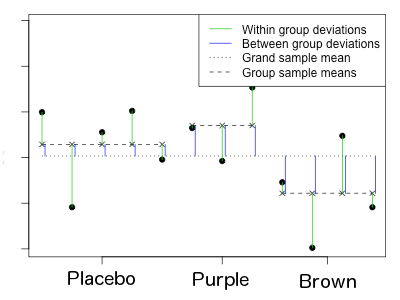
\includegraphics[scale=0.6]{figures/anova-middle-ground-jelly-bean.png}

\end{frame}

%-------------------------------------------------------------------------------
\begin{frame}
\frametitle{Relatively large WITHIN group variation: little apparent difference}

\centering
\(
\sum {\color{blue} \mid}^2 \Big/ \sum {\color{green} \mid}^2
\)

    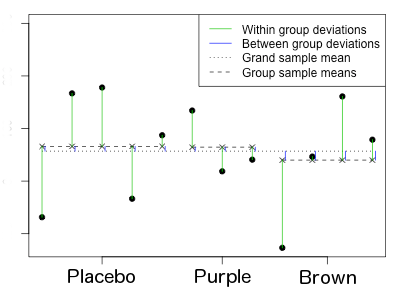
\includegraphics[scale=0.6]{Figures/anova-lots-of-within-group-jelly-bean.png}

\end{frame}

%-------------------------------------------------------------------------------
\begin{frame}
\frametitle{Relatively large BETWEEN group variation: there may be a difference}

\centering
\(
\sum {\color{blue} \mid}^2 \Big/ \sum {\color{green} \mid}^2
\)
    
    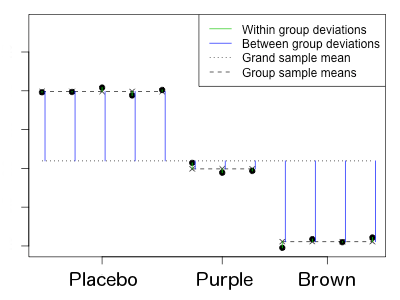
\includegraphics[scale=0.6]{Figures/anova-lots-of-between-group-jelly-bean.png}

\end{frame}

%%%%%%%%%%%%%%%%%%%%%%%%%%%%%%

\begin{frame}
  \frametitle{}

For historical reasons, we use a modification of this ratio called the $F$-statistic:
\[
F = \frac{\sum {\color{blue} \mid}^2 \; \; / \; \; (k - 1)}{\sum {\color{green} \mid}^2 \; \; / \; \; (n - k)}
\hspace{12pt} = \hspace{12pt} \frac{MSG}{MSE}
\]

$k$: \# of groups; $n$: \# of obs.

\pause

\begin{center}
\small
\begin{tabular}{lllrrr}
  \hline
  & Df  & Sum Sq & Mean Sq & F value & Pr($>$F) \\ 
  \hline
  Between groups & k-1 & $\sum {\color{blue}\mid}^2$  & MSG & $F_{obs}$ & $p_{obs}$ \\ 
  Within groups & n-k & $\sum {\color{green}\mid}^2$ & MSE &		 &  \\ 
   \hline
Total			& n-1 & $\sum ({\color{blue}\mid} + {\color{green}\mid})^2$    &                &                &
\end{tabular}
\end{center}

\end{frame}

%%%%%%%%%%%%%%%%%%%%%%%%%%%%%%

\subsection{To identify which means are different, use t-tests and the Bonferroni correction}
\label{mi4}

%%%%%%%%%%%%%%%%%%%%%%%%%%%%%%%%%%%%

\begin{frame}
\frametitle{To identify which means are different, use t-tests and the Bonferroni correction}

\begin{itemize}

\item If the ANOVA yields a significant results, next natural question is: ``Which means are different?"

\item Use t-tests comparing each pair of means to each other, 
\begin{itemize}
\item with a common variance ($MSE$ from the ANOVA table) instead of each group's variances in the 
calculation of the standard error,
\item and with a common degrees of freedom ($df_E$ from the ANOVA table)
\end{itemize}

\item Compare resulting p-values to a modified significance level
\[ \alpha^\star = \frac{\alpha}{K} \]
where $K$ is the total number of pairwise tests

\end{itemize}

\end{frame}

%%%%%%%%%%%%%%%%%%%%%%%%%%%%%%%%%%%%

\begin{frame}

\vfill

\app{4.4 ANOVA}{See the course webpage for details.}

\vfill

\end{frame}

%%%%%%%%%%%%%%%%%%%%%%%%%%%%%%%%%%

\section{Summary}

%%%%%%%%%%%%%%%%%%%%%%%%%%%%%%%%%%%%

\begin{frame}
\frametitle{Summary of main ideas}

\vfill

\begin{enumerate}

\item \nameref{mi1}

\item \nameref{mi2}

\item \nameref{mi3}

\item \nameref{mi4}

\end{enumerate}

\vfill

\end{frame}

%%%%%%%%%%%%%%%%%%%%%%%%%%%%%%%%%%%

\end{document}